\chapter{Analýza problému}

Jako semestrální projekt jsme si ve skupině vybrali ovládání světel lampy na základě různých environmentálních podmínek. Konkrétně se jedná o osvětlení parkoviště mezi budovou FEI a FNO o rozměrech zhruba přibližně 40x60 m. Naše řešení je centralizovaný systém s distribuovanou vizualizací. Za pomoci jednoho PC (případně i Raspberry Pi) zpracováváme data ze světel a senzorů na chtěné hodnoty a následně je posíláme jako příkazy na ovládání světel. Tento počítač pak posílá data pomocí UDP protokolu po síti, na kterou se lze připojit vizualizací. Kdyby se kdokoliv rozhodl tento systém uplatnit a chtěl by použít bezdrátovou komunikaci, pak bude systém spíše distribuovaný, neboť hlavní počítač bude posílat pouze data systému jednotlivých světel. 

Rozhodli jsme se použít senzory VISIC620 od společnosti SICK. Volba padla právě na tento typ senzoru, protože je schopen snímat v podstatě všechny změny environmentálních podmínek. Používáme konkrétně alespoň čtyři senzory pro určení viditelnosti, ze kterých se vytváří průměrná hodnota viditelnosti, dle které systém reaguje na změny. Následně bude systémově ošetřeno, aby se při případném poškození senzoru (tzn. hodnoty se budou výrazně lišit), zobrazilo upozornění ve vizualizaci.\parencite{senzor}

PC je propojeno se světly pomocí kabelů dle druhu světla, případně bezdrátově, dle možnosti daných světel. PC musí být připojeno k wifi za účelem vizualizace.



\begin{figure}[H]
    \centering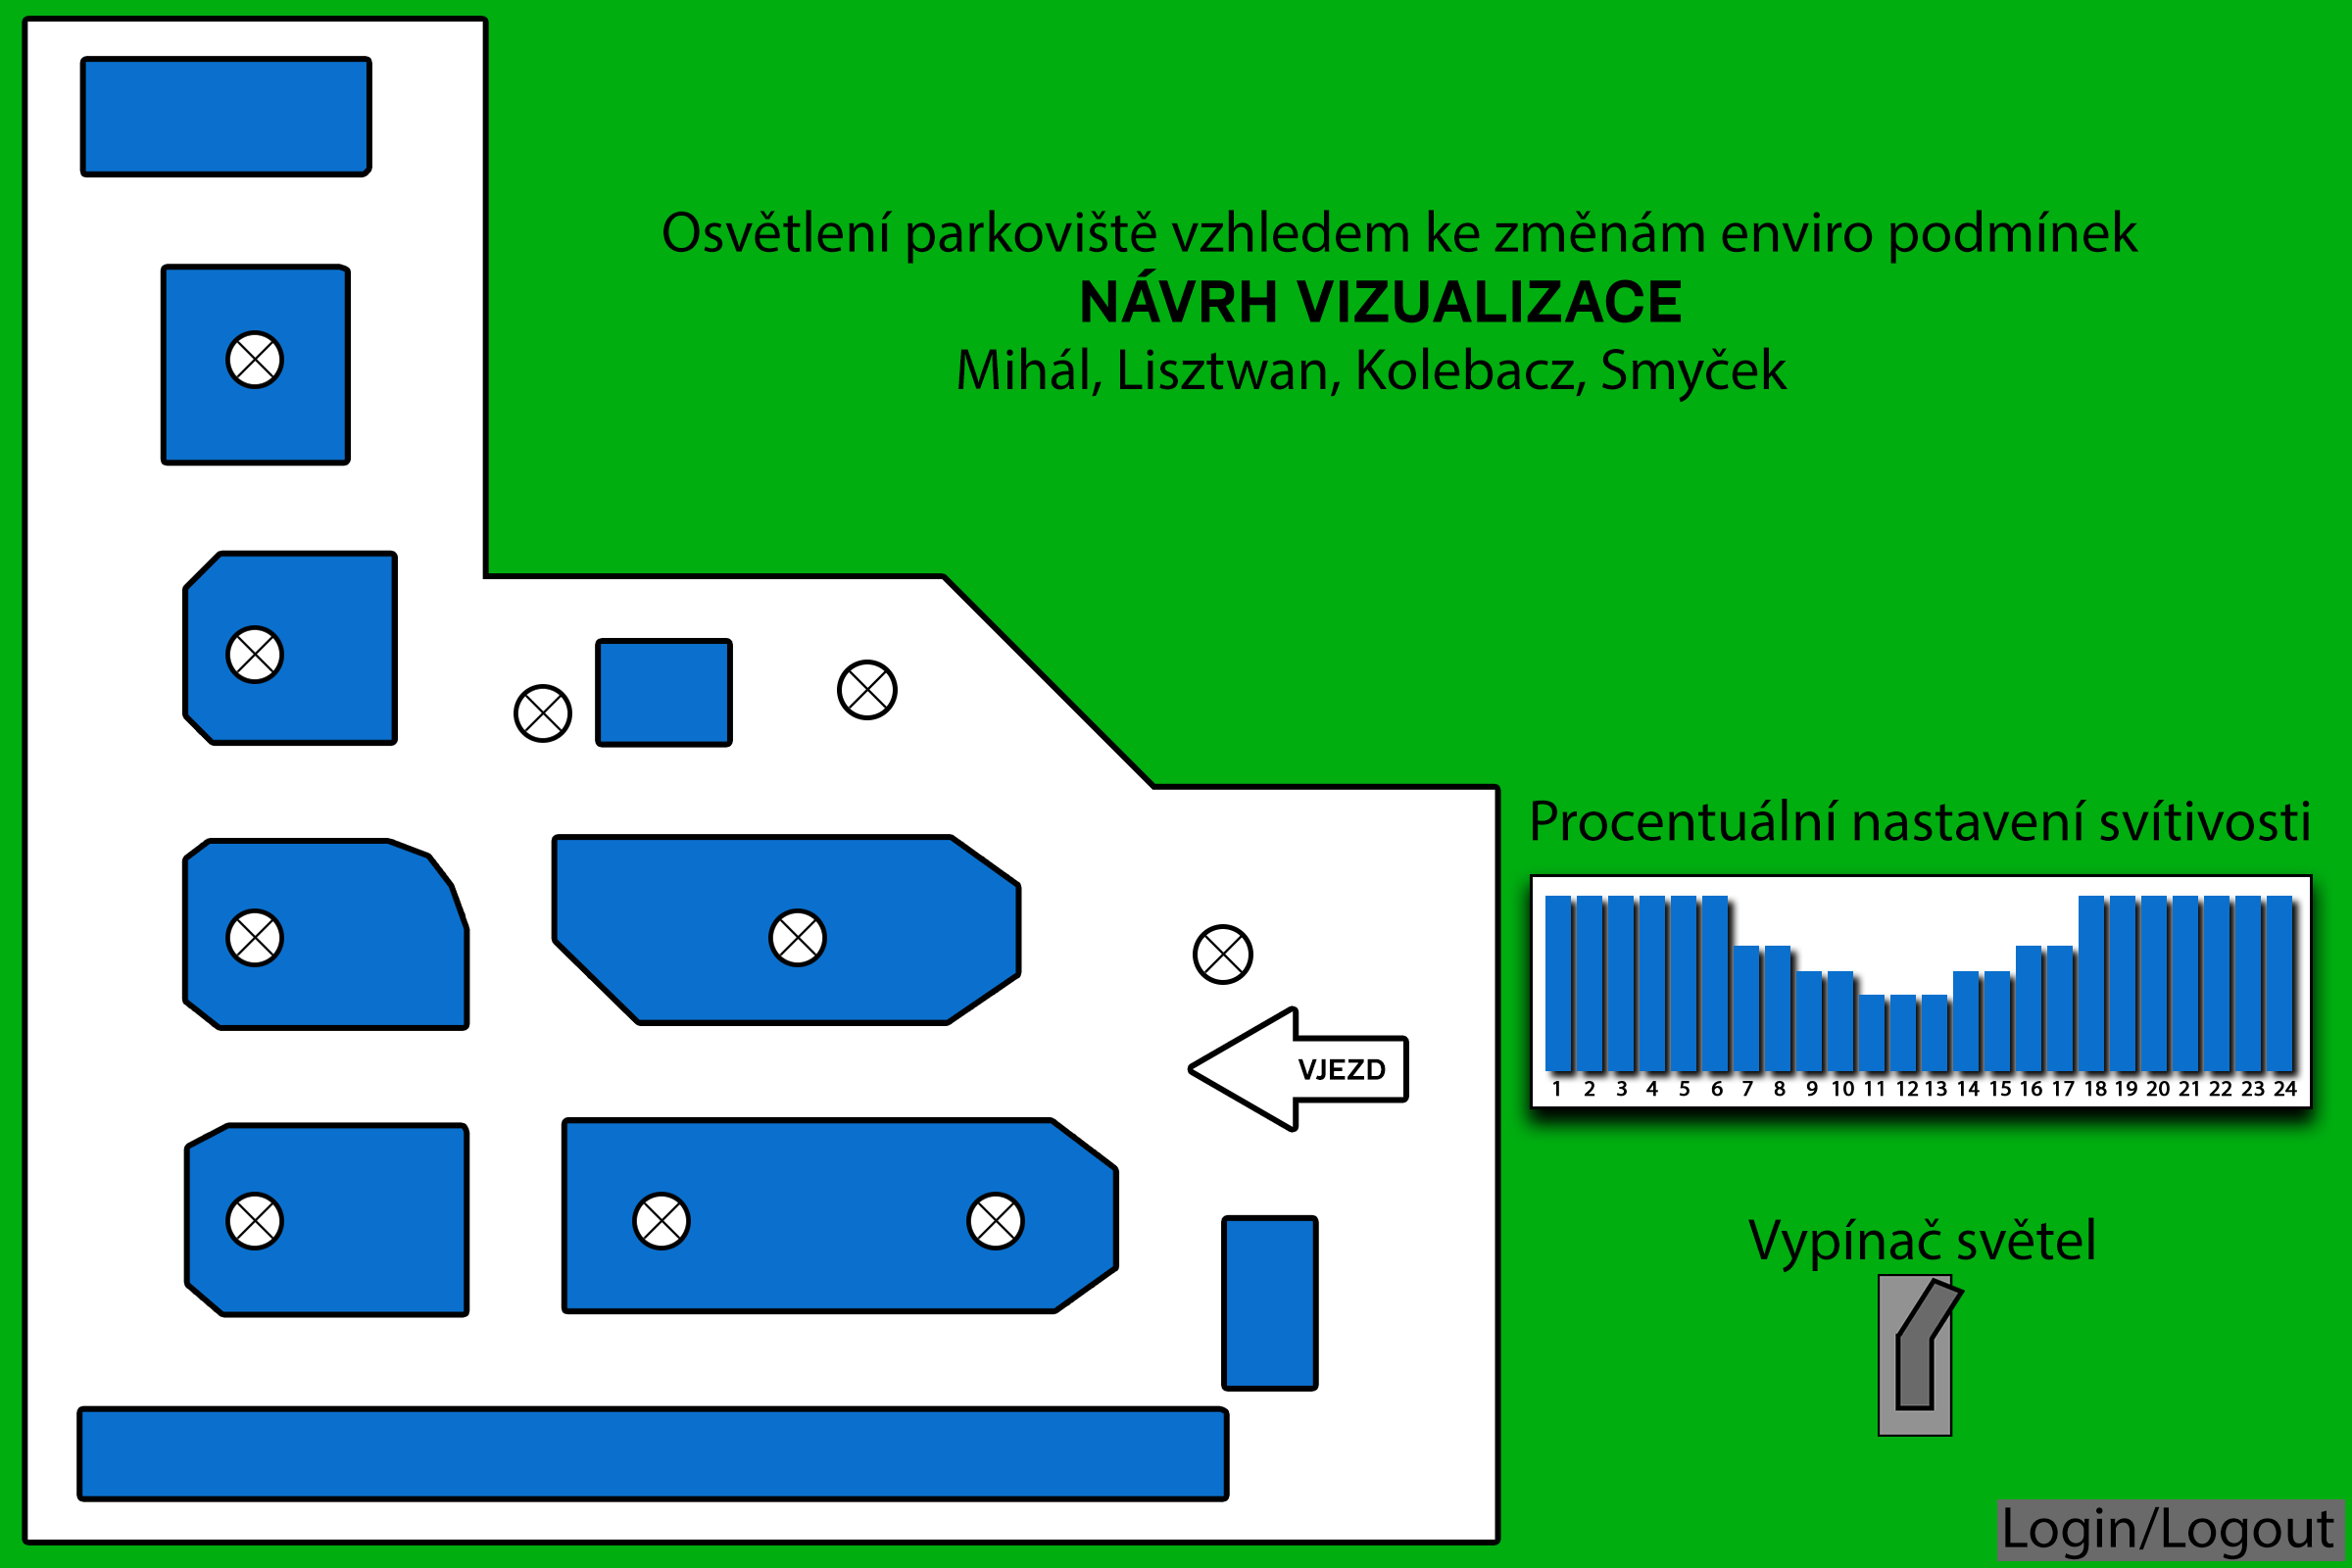
\includegraphics[width=\textwidth]{Figures/Navrh-viz.png}   
    \caption{Prvotní návrh vizualizace -- modře jsou označena místa pro parkování a „žárovičkou“ daná světla (v plné velikosti viz \hyperref[Sec-Prilohy]{Přílohy})}
    \label{Obr-Navrh-viz}
\end{figure}


% \begin{table}[htbp]
% 	\centering
% 	\caption{Definice I/O}
% 	\begin{tabular}{ccccc}
% 		\hline
% 		I/O 
%         & Název proměnné    &Datový typ & Popis \\ \hline
% 		\multirow{3}{*}{I} 
%         & BehLinky          & BOOL      & zapínání/vypínání běhu linky \\
% 		& PaletaVysunuta    & BOOL      & snímač pro vysunutí palety \\ 
% 		& Zrychleni   		& UINT      & volba rychlosti pásu \\ \hline
%         \multirow{6}{*}{O} 
% 		& Snimac            & BOOL      & snímač výrobků \\
% 		& AplikatorFolie    & BOOL      & indikátor aplikátoru folie \\
% 		& HorkovzdusnyFen   & BOOL      & indikátor horkovzdušného fénu \\
% 		& VysouvaciRameno   & BOOL      & indikátor vysouvacího ramena \\
% 		& PocetVyrobku      & UINT      & počítání výrobků \\
% 		& PocetPalet        & UINT      & počítání palet \\ \hline
% 	\end{tabular}
%     \label{Tab-IO}
% \end{table}


\endinput
